\section{Sectors, order, and confinement}\label{sec:sectors}

We first reduce the possible ends of a bigeodesic to countably many pairs of
opposite sectors.  Within each sector, planar order will let us obtain a
uniform statement about every ray from estimates for only four fixed
functionals.  All assertions below are made on the event of finite
uniqueness and simultaneous ray asymptotics in \Cref{thm:structure}, together
with \Cref{lem:uniform-metric}.  Whenever a countable deterministic collection
of functionals is specified, we also impose the fixed-functional conclusions
of \Cref{thm:structure} for that collection.

\begin{lemma}[Opposite functionals]\label{lem:opposite}
Let an oriented bigeodesic pass through $z$, and let $p^+$ and $p^-$ be its
two rays starting at $z$.  Then, for every $w\in\Z^2$,
\begin{equation}\label{eq:bigeodesic-sum}
 B_{p^+}(z,w)+B_{p^-}(z,w)\leq 0.
\end{equation}
Consequently $\rho_{p^-}=-\rho_{p^+}$.  Moving the base point along the
bigeodesic does not change either functional or either Busemann function.
For any deterministic countable set $D\subset C$, almost surely no
bigeodesic has an end whose functional belongs to $D$.
\end{lemma}

\begin{proof}
For vertices $p_i^+$ and $p_j^-$ on opposite arms, optimality and the triangle
inequality give
\[
 T(z,p_i^+)+T(z,p_j^-)
 =T(p_i^+,p_j^-)
 \leq T(w,p_i^+)+T(w,p_j^-).
\]
Subtract the right-hand terms and let $i,j\to\infty$.  This proves
\eqref{eq:bigeodesic-sum}.  Additivity and asymptotic linearity imply that
its left-hand side is
\[
 (\rho_{p^+}+\rho_{p^-})(w-z)+o(|w|)
 \qquad (|w|\to\infty).
\]
Putting $w=z+ne_k$ and $w=z-ne_k$, dividing by $n$, and letting
$n\to\infty$, for $k=1,2$, proves that the sum of the functionals vanishes.
The assertion about moving the base point follows from tail invariance in
\Cref{lem:busemann-basic}.

The exclusion of a deterministic countable set is \Cref{cor:fixed-label}.
\end{proof}

We use rotations and reflections preserving $\Z^2$ when choosing coordinates.
In any such coordinates, $e_1$ is horizontal and $e_2$ is vertical.
The symmetry of the law implies the same symmetry of $m$ and $C$; in
particular $-C=C$.  To see the latter assertion directly from the structural
input, reflect the unique ray for a fixed $\rho\in C$.  The reflected
environment has the same law, and its ray has functional $-\rho$, which must
belong to the deterministic set $C$.

\begin{lemma}[Countably many charts]\label{lem:charts}
There is a deterministic countable set $D\subset C$, symmetric under
negation, and a countable family of charts with the following properties.
Each chart is specified by a choice of lattice coordinates and a compact
arc $J$ of the dual unit circle, whose distinct endpoints $\rho_\ell,
\rho_r$ belong to $C$.  Set $I=C\cap J$.  There is $c>0$ such that
\begin{equation}\label{eq:chart-contact-sector}
 d_2\geq c
 \quad\text{for every }\rho\in J\text{ and every }d\in A(\rho).
\end{equation}
The coordinate
\[
 r(\rho)=\rho(e_1)
\]
is one-to-one on $J$ and orders it from $\rho_\ell$ to $\rho_r$ with
$r(\rho_\ell)<r(\rho_r)$.  Every member of $C\setminus D$ belongs to the
relative interior of such a chart arc.  Almost surely, every bigeodesic
can therefore be oriented so that its upper functional belongs to the
interior of one of these charts and its lower functional is its negative.
\end{lemma}

\begin{proof}
Let $K=\{x:m(x)\leq1\}$, and let
$K^*=\{\rho:\rho(x)\leq m(x)\text{ for all }x\}$ be the dual unit ball.
For $\rho\in\partial K^*$ the exposed face
\[
 F_\rho=\{x\in K:\rho(x)=1\}
\]
is a point or a line segment.  Its radial image is $A(\rho)$.  If this
image contains two directions, it is a nondegenerate closed circular arc.
The relative interiors of these arcs are disjoint for distinct $\rho$:
a direction in such an interior corresponds to the relative interior of a
nondegenerate face of $K$, whose supporting line, and hence its normalized
functional, is unique.  Each nondegenerate arc contains a rational angle.
Thus only countably many functionals have more than one contact direction.

There are also only countably many members of $C$ that are isolated on
at least one circular side.  Indeed, they are endpoints of components of
$\partial K^*\setminus C$, with the finite-set cases included.  The open
components are disjoint and each contains a point of a fixed countable
dense subset of the circle.

Consider a remaining $\rho\in C$, so that $A(\rho)=\{d\}$ and $C$
accumulates at $\rho$ from both circular sides.  A lattice rotation makes
$d_2>0$.  The contact correspondence is upper semicontinuous: if
$\rho_n\to\rho$ and $d_n\in A(\rho_n)$ with $d_n\to d'$, then
$m(d')=\rho(d')$.  Compactness of the unit circle therefore supplies an
open boundary neighborhood of $\rho$ on which every contact has vertical
coordinate at least some $c>0$.

Choose once and for all a countable dense subset $D_0$ of $C$.  In the
neighborhood just obtained, choose one point of $D_0$ on either side of
$\rho$.  The compact boundary arc joining them through $\rho$ can be taken
inside that neighborhood.  There are only countably many pairs from
$D_0$ and finitely many choices of lattice coordinates, so all such arcs
form a countable family.  For $D$ take the union of $D_0$, the two
countable exceptional sets described above, and their negatives.

For completeness, suppose two chart points $\rho,\lambda$ had the same
horizontal coordinate and $\lambda(e_2)>\rho(e_2)$.  Choosing any
$d\in A(\rho)$, for which $d_2>0$, would give
$\lambda(d)>\rho(d)=m(d)$, contrary to $\lambda\in K^*$.
The same argument shows that each chart point is the top endpoint of
the vertical section of $K^*$ at its horizontal coordinate.
The continuous horizontal coordinate is thus injective on the arc and
strictly monotone along it.  Orient $J$ so that it increases.  On the
opposite lower arc, the horizontal coordinate again increases from left
to right; negation reverses the order of the corresponding labels.

Finally, \Cref{lem:opposite} excludes $D$ simultaneously and identifies
the opposite end.  The contact restriction implies that rays of the
chosen upper label tend to height $+\infty$, and those of the negative
label tend to height $-\infty$.  This gives the claimed orientation.
\end{proof}

Fix one chart for the rest of this section.  We call a functional of a ray
its \emph{label}; an upper label belongs to $I$ and a lower label belongs to
$-I$.  Since a simple ray eventually leaves every finite set, its contact
restriction and \eqref{eq:chart-contact-sector} show that its height tends
to the appropriate infinity.  No monotonicity of height along the ray is
asserted.

We will use the following elementary planar fact.  Two disjoint polygonal
arcs connecting the lower and upper boundary lines of a strip, with their
interiors in the open strip, have their endpoints in the same left-to-right
order on the two boundary lines.  One way to prove this is to put the
finite arcs inside a sufficiently wide rectangle and apply the Jordan
curve theorem to one arc and either of the two boundary routes joining
its endpoints.  Endpoints in reversed order lie on opposite sides of that
Jordan curve, so the other arc must cross the first.  The same conclusion
holds for finite walks, by erasing loops before applying this argument.
For nearest-neighbor lattice paths, a planar intersection always yields a
common lattice vertex: interiors of perpendicular unit edges do not cross,
and overlapping unit edges have common endpoints.

\begin{lemma}[Local ray order]\label{lem:ray-order}
Two upper rays with disjoint tails have a stable left-to-right order at
their first visits to the horizontal rows $\{x_2=N\}$ as $N\to\infty$.
If $p$ is to the left of $q$ in this order, then
\begin{equation}\label{eq:ray-order}
 r(\rho_p)\leq r(\rho_q).
\end{equation}
In particular, distinct labels give disjoint tails and strictly ordered
first arrivals, in the order of increasing $r$.  For lower rays the same
statements hold as $N\to-\infty$, again with left-to-right order given by
increasing horizontal coordinate of the lower functional.
\end{lemma}

\begin{proof}
If two rays meet infinitely often, choose a shared vertex beyond their
finite initial portions.  The geodesic segments from that vertex to every
later common vertex agree by finite uniqueness.  The later common vertices
escape to infinity, so the two tails agree.  Tail invariance of the
Busemann function then gives equality of their labels.  Thus distinct
labels have only finitely many common vertices.

Suppose the tails of $p$ and $q$ are disjoint.  Choose an integer height
$h$ above both starting sites, above all intersections, and above finite
prefixes preceding the disjoint tails.  After their respective last visits
to row $h$, both rays stay strictly above that row.  For sufficiently large
$N$, their first visits to row $N$ occur after those last visits, since the
prefixes ending at the last visits are finite.  The intervening arcs are
disjoint strip crossings.  Their order on row $N$ therefore agrees with
the fixed order of the last visits to row $h$.  This proves stabilization.

Assume this stable order is $p$ to the left of $q$.  For a positive integer
$n$, set $u=(-n,0)$ and $v=(n,0)$.  Let $\gamma_j$ be the concatenation of
the finite geodesic from $v$ to $p_j$ and the tail of $p$ after $p_j$.
This concatenation is used as a walk; it need not be a ray or be simple.
Define
\[
 \delta_j=T(v,p_j)-B_p(v,p_j)\geq0.
\]
Since
$B_p(v,p_j)=B_p(v,p_0)+T(p_0,p_j)$, the definition of $B_p$ implies
$\delta_j\to0$ for this fixed $v$.  Every vertex $w$ of $\gamma_j$ satisfies
\begin{equation}\label{eq:near-calibration}
 0\leq T(v,w)-B_p(v,w)\leq\delta_j.
\end{equation}
On the initial geodesic this follows by decomposing its cost and the
Busemann increment at $w$, with the remaining deficit nonnegative.
On the tail it follows from the triangle inequality and exact calibration
of $p[p_j,w]$.  Define $\xi_j$ in the same way by joining $u$ to $q_j$
and then following $q$, and write its error as $\delta'_j\to0$.

We next control all row-zero visits of these walks, including visits very
far from the origin.  The horizontal directions are outside both contact
sets, so
\[
 \gamma=
 \min_{\lambda\in\{\rho_p,\rho_q\},\,\sigma\in\{-1,1\}}
 \bigl(m(\sigma e_1)-\lambda(\sigma e_1)\bigr)>0.
\]
Write $a_p(x)=B_p(0,x)-\rho_p(x)$, and define $a_q$ similarly.  Given
$\eps>0$, the uniform metric estimate and these two rooted asymptotics
give a finite $K_\eps$ such that, for all lattice sites $x,y$,
\begin{align*}
 |T(x,y)-m(y-x)|&\leq\eps(|x|+|y|)+K_\eps,\\
 |a_p(x)|+|a_q(x)|&\leq\eps|x|+K_\eps.
\end{align*}
For $w=(t,0)$ with $d=|w-v|\geq n/2$, we have
$|v|+|w|\leq2n+d\leq5d$.  Additivity therefore gives the explicit bound
\begin{equation}\label{eq:row-deficit}
 T(v,w)-B_p(v,w)
 \geq (\gamma-10\eps)d-3K_\eps.
\end{equation}
The identical estimate holds with $u,q$ in place of $v,p$.  Choose
$\eps<\gamma/40$ first, and then $n$ so large that
$3K_\eps\leq\gamma n/8$.  The right-hand side of
\eqref{eq:row-deficit} is at least $\gamma d/2\geq\gamma n/4$.
For this fixed $n$, choose $j$ so large that both approximate-calibration
errors are smaller than $\gamma n/4$.  It follows that every row-zero
visit of $\gamma_j$ has horizontal coordinate in $(n/2,3n/2)$, whereas
every such visit of $\xi_j$ lies in $(-3n/2,-n/2)$.

Both walks eventually follow their exact upward tails.  Their last
row-zero visits thus exist and have the order $\xi_j,\gamma_j$.
Choose a row $N$ above the finite joining paths, the discarded original
prefixes $p[p_0,p_j]$ and $q[q_0,q_j]$, and the prefixes ending at these last
row-zero visits, and high enough for the stable order of $p,q$.
The first visits of the two walks to this row occur on their exact tails
and have the opposite order $\gamma_j,\xi_j$.  Their portions from the
last row-zero visits to these first row-$N$ visits are strip crossings.
The planar fact gives a common vertex $w_j$.

At that vertex, domination by the metric and \eqref{eq:near-calibration}
give
\begin{align*}
 B_p(u,v)
 &=B_p(u,w_j)-B_p(v,w_j)\\
 &\leq T(u,w_j)-T(v,w_j)+\delta_j\\
 &\leq B_q(u,w_j)-B_q(v,w_j)+\delta_j+\delta'_j\\
 &=B_q(u,v)+\delta_j+\delta'_j.
\end{align*}
Let $j\to\infty$ with $n$ fixed.  We obtain $B_p(u,v)\leq B_q(u,v)$.
Finally, the rooted asymptotics at $u$ and $v$ give
\[
 B_p(u,v)=2n\rho_p(e_1)+o(n),\qquad
 B_q(u,v)=2n\rho_q(e_1)+o(n).
\]
Division by $2n$ proves \eqref{eq:ray-order}.  If the labels are distinct,
injectivity of $r$ makes the order strict.  Reflection in the horizontal
axis proves the lower-ray version; this reflection preserves $e_1$, so it
also preserves the horizontal parameter used in that version.
\end{proof}

Choose $s>0$ sufficiently small that every upper contact in the chart
satisfies $d_2>2s|d_1|$, and every lower contact satisfies
$-d_2>2s|d_1|$.  This is possible by compactness and
\eqref{eq:chart-contact-sector}.  For $z\in\Z^2$ and $H\geq0$, define the
closed convex offset cones
\begin{equation}\label{eq:offset-cones}
 Q^\pm(z,H)=
 \{w\in\R^2:\ \pm(w_2-z_2)\geq s|w_1-z_1|-H\}.
\end{equation}

\begin{proposition}[Uniform confinement of all rays]\label{prop:cone}
Almost surely there is a finite $H(z)\geq1$ for every $z\in\Z^2$ such that
every upper ray from $z$ lies in $Q^+(z,H(z))$ and every lower ray from $z$
lies in $Q^-(z,H(z))$.  Moreover, for every fixed $L<\infty$,
\begin{equation}\label{eq:uniform-cone-offset}
 \max_{|z|\leq Ln}H(z)=o(n)\qquad(n\to\infty).
\end{equation}
These statements hold simultaneously for every ray in the chart; no
uniform rate of Busemann convergence over the intermediate labels is
required.
\end{proposition}

\begin{proof}
Let
$\Lambda=\{\rho_\ell,\rho_r,-\rho_\ell,-\rho_r\}$.
For each of these four deterministic functionals, \Cref{thm:structure}(iii)
provides a unique ray $g^\lambda_z$ from every vertex $z$ and a common
Busemann function $B_\lambda$.  Let $\sigma_\lambda=1$ for the upper
endpoints and $\sigma_\lambda=-1$ for the lower endpoints.  Define
\begin{equation}\label{eq:endpoint-offset}
 H(z)=1+\max_{\lambda\in\Lambda}
 \sup_{w\in g^\lambda_z}
 \bigl(s|w_1-z_1|-\sigma_\lambda(w_2-z_2)\bigr)_+.
\end{equation}
Each supremum is finite.  Indeed, the limit directions of this endpoint
ray lie strictly inside its cone of slope $2s$, and translating the
origin to its fixed starting point does not change its limit directions.
Outside a finite prefix the displayed positive part is therefore zero.

We prove \eqref{eq:uniform-cone-offset} first for these endpoint rays.
Put $a_\lambda(x)=B_\lambda(0,x)-\lambda(x)=o(|x|)$.  If
$w\in g^\lambda_z$, calibration gives
\begin{equation}\label{eq:endpoint-calibration}
 T(z,w)=B_\lambda(z,w)
 =\lambda(w-z)+a_\lambda(w)-a_\lambda(z).
\end{equation}
Fix $L$ and $\eta>0$.  Whenever $|z|\leq Ln$ and $d=w-z$ satisfies
$|d|\geq\eta n$, we have
\[
 |z|+|w|\leq 2Ln+|d|
 \leq(1+2L/\eta)|d|.
\]
The uniform metric approximation, the four rooted asymptotics, and
\eqref{eq:endpoint-calibration} thus imply
\begin{equation}\label{eq:endpoint-gap-small}
 \sup_{
 \substack{\lambda\in\Lambda,\ |z|\leq Ln,\ w\in g^\lambda_z\\
                 |w-z|\geq\eta n}}
 \frac{m(w-z)-\lambda(w-z)}{|w-z|}\longrightarrow0.
\end{equation}
To make the uniformity explicit, bound each rooted error by
$\eps|x|+K_\eps$ and the metric error by
$\eps(|z|+|w|)+K_\eps$.  The quotient in
\eqref{eq:endpoint-gap-small} is then at most
$2\eps(1+2L/\eta)+3K_\eps/(\eta n)$; take $n\to\infty$ and then
$\eps\downarrow0$.

For each $\lambda\in\Lambda$, the continuous function
$m(d)-\lambda(d)$ has a strictly positive minimum on
\[
 \{d\in S^1:\ \sigma_\lambda d_2\leq s|d_1|\},
\]
because all its zeros lie strictly inside the cone of slope $2s$.
Taking the minimum over the four functionals preserves positivity.
It follows from \eqref{eq:endpoint-gap-small} that, for all sufficiently
large $n$, every endpoint-ray displacement with $|d|\geq\eta n$ lies
in the unshifted cone of slope $s$.  For the remaining displacements,
\[
 \bigl(s|d_1|-\sigma_\lambda d_2\bigr)_+
 \leq(s+1)|d|<(s+1)\eta n.
\]
Consequently the maximum in \eqref{eq:uniform-cone-offset} is at most
$1+(s+1)\eta n$ eventually.  Letting $\eta\downarrow0$ proves that
equation for the $H(z)$ in \eqref{eq:endpoint-offset}.

It remains to trap every intermediate ray with exactly this offset.
Fix $z$ and an upper ray $p$ with
$r(\rho_\ell)<r(\rho_p)<r(\rho_r)$.  Write
$a=g^{\rho_\ell}_z$, $b=g^{\rho_r}_z$, and $Q=Q^+(z,H(z))$.
The bounding rays lie in $Q$.  Finite uniqueness implies that they have
a common finite prefix ending at a vertex $v$, and then disjoint tails.
Indeed, a reunion after their first split would give two finite
geodesics from $z$ to the reunion vertex.  Their common prefix is finite
because their labels differ.

Suppose, for a contradiction, that $p$ visits a vertex $w\notin Q$.
Choose an integer $N$ above the heights of the entire common prefix of
$a,b$, above the finite prefix of $p$ ending at $w$, and large enough
for the three pairwise orders in \Cref{lem:ray-order} to have stabilized.
Let $a_N,b_N,p_N$ denote their first arrivals on row $N$.  They are
strictly ordered as
\[
 (a_N)_1<(p_N)_1<(b_N)_1.
\]
Each first-arrival path lies strictly below that row until its endpoint.
The two arcs $a[v,a_N]$ and $b[v,b_N]$, together with the horizontal
segment $[a_N,b_N]$, form a simple closed polygonal curve $\mathcal J$.
Let $\mathcal D$ be its bounded Jordan domain.  The curve lies in $Q$,
including its top segment by convexity.  Since a bounded Jordan domain
is contained in the convex hull of its boundary, $\mathcal D\subset Q$.

The common prefix $a[z,v]=b[z,v]$ need not lie in $\mathcal D$; viewed
from the Jordan curve it may form a slit on either side.  The following
first-arrival argument treats that possibility explicitly; see
\Cref{fig:trapping}.  The last
edge into $p_N$ is vertical from below.  Since $p_N$ is in the relative
interior of the top segment, the part of that edge sufficiently close
to $p_N$ lies inside $\mathcal D$.  Starting at $w\notin Q$, the ray
therefore passes from outside $\mathcal D$ to its inside before its
first row-$N$ arrival.  It cannot enter through the top segment, since
that would already be a visit to row $N$.  Hence, after $w$, it meets
one of the two bounding arcs at a lattice vertex $u$, possibly $u=v$.
Both its prefix $p[z,u]$ and the corresponding bounding prefix are
finite geodesics.  Uniqueness makes them identical.  The bounding
prefix is contained in $Q$, whereas $p[z,u]$ contains $w\notin Q$,
a contradiction.  This argument also rules out departures made before
the bounding rays split.

\begin{figure}[tbp]
\centering
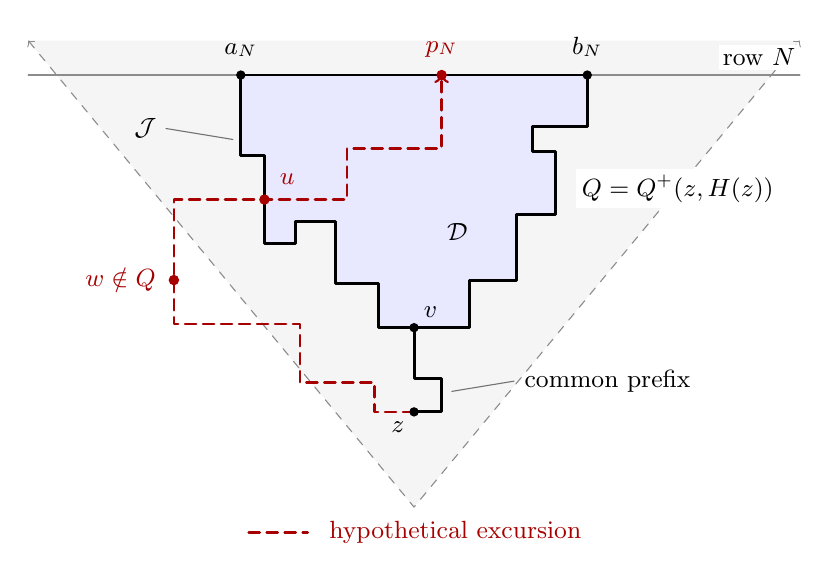
\begin{tikzpicture}[x=1cm,y=.93cm,font=\small,
  line cap=round,line join=round]
  \fill[black!4] (0,-1.3)--(-4.9,5.07)--(4.9,5.07)--cycle;
  \draw[black!45,dashed,<->] (-4.9,5.07)--(0,-1.3)--(4.9,5.07);
  \fill[blue!9!white]
    (0,1.15)--(-.45,1.15)--(-.45,1.75)--(-1,1.75)
    --(-1,2.6)--(-1.5,2.6)--(-1.5,2.3)--(-1.9,2.3)
    --(-1.9,3.5)--(-2.2,3.5)--(-2.2,4.6)
    --(2.2,4.6)--(2.2,3.9)--(1.5,3.9)--(1.5,3.55)
    --(1.8,3.55)--(1.8,2.7)--(1.3,2.7)--(1.3,1.8)
    --(.7,1.8)--(.7,1.15)--cycle;
  \draw[black!45] (-4.9,4.6)--(4.9,4.6);
  \draw[line width=.95pt] (-2.2,4.6)--(2.2,4.6);
  \node[anchor=south east,fill=white,inner sep=1.5pt]
    at (4.9,4.66) {row $N$};

  \draw[line width=1.05pt]
    (0,0)--(.35,0)--(.35,.45)--(0,.45)--(0,1.15);
  \draw[black!55] (1.27,.42)--(.48,.28);
  \node[anchor=west] at (1.28,.42) {common prefix};

  \draw[line width=1.05pt]
    (0,1.15)--(-.45,1.15)--(-.45,1.75)--(-1,1.75)
    --(-1,2.6)--(-1.5,2.6)--(-1.5,2.3)--(-1.9,2.3)
    --(-1.9,3.5)--(-2.2,3.5)--(-2.2,4.6);
  \draw[line width=1.05pt]
    (0,1.15)--(.7,1.15)--(.7,1.8)--(1.3,1.8)
    --(1.3,2.7)--(1.8,2.7)--(1.8,3.55)--(1.5,3.55)
    --(1.5,3.9)--(2.2,3.9)--(2.2,4.6);

  \draw[red!65!black,line width=.95pt,dash pattern=on 4pt off 2.5pt,->]
    (0,0)--(-.5,0)--(-.5,.4)--(-1.45,.4)--(-1.45,1.2)
    --(-3.05,1.2)--(-3.05,2.9)--(-.85,2.9)--(-.85,3.6)
    --(.35,3.6)--(.35,4.6);
  \fill (0,0) circle (1.7pt) (0,1.15) circle (1.7pt)
    (-2.2,4.6) circle (1.7pt) (2.2,4.6) circle (1.7pt);
  \fill[red!65!black] (-3.05,1.8) circle (1.9pt)
    (-1.9,2.9) circle (1.9pt) (.35,4.6) circle (1.9pt);
  \node[below left] at (0,0) {$z$};
  \node[above right] at (0,1.15) {$v$};
  \node[above=3pt] at (-2.2,4.6) {$a_N$};
  \node[above=3pt] at (2.2,4.6) {$b_N$};
  \node[above=3pt,text=red!65!black] at (.35,4.6) {$p_N$};
  \node[left=3pt,text=red!65!black] at (-3.05,1.8) {$w\notin Q$};
  \node[above right=2pt,text=red!65!black] at (-1.9,2.9) {$u$};
  \node at (.55,2.45) {$\mathcal D$};
  \node[fill=white,inner sep=2pt] at (3.35,3.05) {$Q=Q^+(z,H(z))$};
  \draw[black!55] (-3.15,3.87)--(-2.3,3.72);
  \node[left] at (-3.15,3.87) {$\mathcal J$};
  \draw[red!65!black,line width=.95pt,dash pattern=on 4pt off 2.5pt]
    (-2.1,-1.65)--(-1.35,-1.65);
  \node[anchor=west,text=red!65!black] at (-1.2,-1.65)
    {hypothetical excursion};
\end{tikzpicture}
\caption{First-arrival trapping, schematically, in $Q=Q^+(z,H(z))$.
The bounding arcs from the split $v$ to $a_N,b_N$, together with the row
segment, form $\mathcal J$ and enclose $\mathcal D\subset Q$.
The common prefix from $z$ need not lie in $\mathcal D$.
A hypothetical intermediate ray visiting $w$ outside the cone must
contact a bounding arc at $u$ before its first arrival at
$p_N\in(a_N,b_N)$, contradicting finite uniqueness. The dashed excursion
depicts this contradiction; no height monotonicity is assumed.}
\label{fig:trapping}
\end{figure}


Thus every intermediate upper ray is in $Q$.  Rays with an endpoint
label are the unique endpoint rays.  Reflection proves the same
statement for lower rays.  The reasoning was deterministic on the
single event already specified and applied to an arbitrary ray, so it
establishes the simultaneous all-ray assertion.
\end{proof}

\begin{lemma}[Crossing from separated sites]\label{lem:crossing}
Let $x_1<y_1$, and suppose upper rays $p$ from $x$ and $q$ from $y$ satisfy
\[
 p\subset Q^+(x,H_x),\qquad q\subset Q^+(y,H_y).
\]
If
\begin{equation}\label{eq:crossing-separation}
 s(y_1-x_1)>H_x+H_y+|x_2-y_2|
\end{equation}
and $r(\rho_p)>r(\rho_q)$, then the rays intersect.  The same assertion
holds for two lower rays in the corresponding lower cones, with the
horizontal coordinates of their lower labels in place of $r(\rho_p)$
and $r(\rho_q)$.
\end{lemma}

\begin{proof}
For upper rays put $h=\max(x_2,y_2)$.  Both rays have a last visit to
row $h$, because they tend upwards.  Call the two last vertices
$\widehat x,\widehat y$.  The cone bounds give
\[
 |\widehat x_1-x_1|\leq\frac{h-x_2+H_x}{s},\qquad
 |\widehat y_1-y_1|\leq\frac{h-y_2+H_y}{s}.
\]
Since $(h-x_2)+(h-y_2)=|x_2-y_2|$,
\eqref{eq:crossing-separation} implies
$\widehat x_1<\widehat y_1$.  If the rays did not intersect, their
portions from these last visits to their first visits to a sufficiently
high row would be disjoint strip crossings.  Their order there would
remain $p,q$, contradicting \Cref{lem:ray-order} and the strict reverse
order of their labels.  For lower rays use
$h=\min(x_2,y_2)$ and the last visits before departure towards height
$-\infty$.  The same estimates and the lower form of
\Cref{lem:ray-order} apply.
\end{proof}

In particular, the separation required on a common horizontal row is
linear in the sum of the offsets.  Heights differing by a bounded
amount only add that amount to the numerator in
\eqref{eq:crossing-separation}.  For fixed sites $u,v$ and sites
$y=(N,h)$ on any fixed horizontal row, \Cref{prop:cone} gives
$H(y)=o(N)$.  Thus for all sufficiently large $N$ the crossing criterion
applies to every reverse-ordered pair of rays from $u,y$, and also to
every such pair from $v,y$.  This simultaneous choice will be useful
when comparing whole ranges of Busemann values.
